\documentclass[letterpaper, **24pt**]{article}
\usepackage{mathtools}
\usepackage[top=2in, bottom=1.5in, left=1in, right=1in]{geometry}
\usepackage{graphicx}
\usepackage[normalem]{ulem}
\usepackage{fancyhdr}
\usepackage{enumerate}
\usepackage{setspace}
\usepackage[T1]{fontenc} 
\usepackage{lmodern}
\usepackage{breqn}
\usepackage[compact]{titlesec} 
\pagestyle{fancyplain}


\lhead{ECON 485 - Econometrics I}

\rhead{Group 1}

\includeonly{introduction, dataoverview, model, regresults, sumstat, varlist, results, litreview, conclusion}

\begin{document}

\title{Wal-Mart and Obesity}
\author{A. Shawn Bandy, Tony Bui, Vincent Larouche, Matthew Pinchback}
\date{May 9\textsuperscript{th}, 2013}
\maketitle
\fontsize{12bp}{14bp}\selectfont

\begin{abstract}
The Center for Disease Control (CDC) estimates 32 percent of American men and 35 percent of women are obese as of 2010.  In 2012, medical costs associated with obesity were estimated by the CDC to be 190 million dollars.\footnote{Jens Ludwig, et al. Neighborhoods, Obesity, and Diabetes. New England Journal of Medicine 365 No 16. http://dx.doi.org/10.1056/NEJMsa1103216}  Wal-Mart Stores, Inc. is a multinational discount retailer with approximately 3000 "Supercenters" in the United States.   Wal-Mart Supercenter stores average 197,000 square feet and provide full-service supermarkets.  Grocery accounts for 55\% of 274 million dollars in net U.S. sales.\footnote{Wal-Mart Stores Inc., 2012 Annual Report, http://az204679.vo.msecnd.net/media/documents/2013-annual-report_130108806067963477.pdf Accessed May 09 2013. }  We explore the possible relationship between the relative concentration of Wal-Mart stores and the obesity rate at the county level.
\end{abstract}
\newpage


\begin{doublespace}
\begingroup
	\section{Introduction and Motivation}\hfill\\
		\let\clearpage\relax
			\fontsize{12bp}{14bp}\selectfont
\subsection{Motivation} 
The motivation for this paper could be best illustrated by the following two maps:\footnote{Source: http://www.cdc.gov/obesity/data/adult.html}\footnote{Source: http://www.zook.info/Wal-Mart/Figure2-2-US-distribution-by-store-type.jpg}

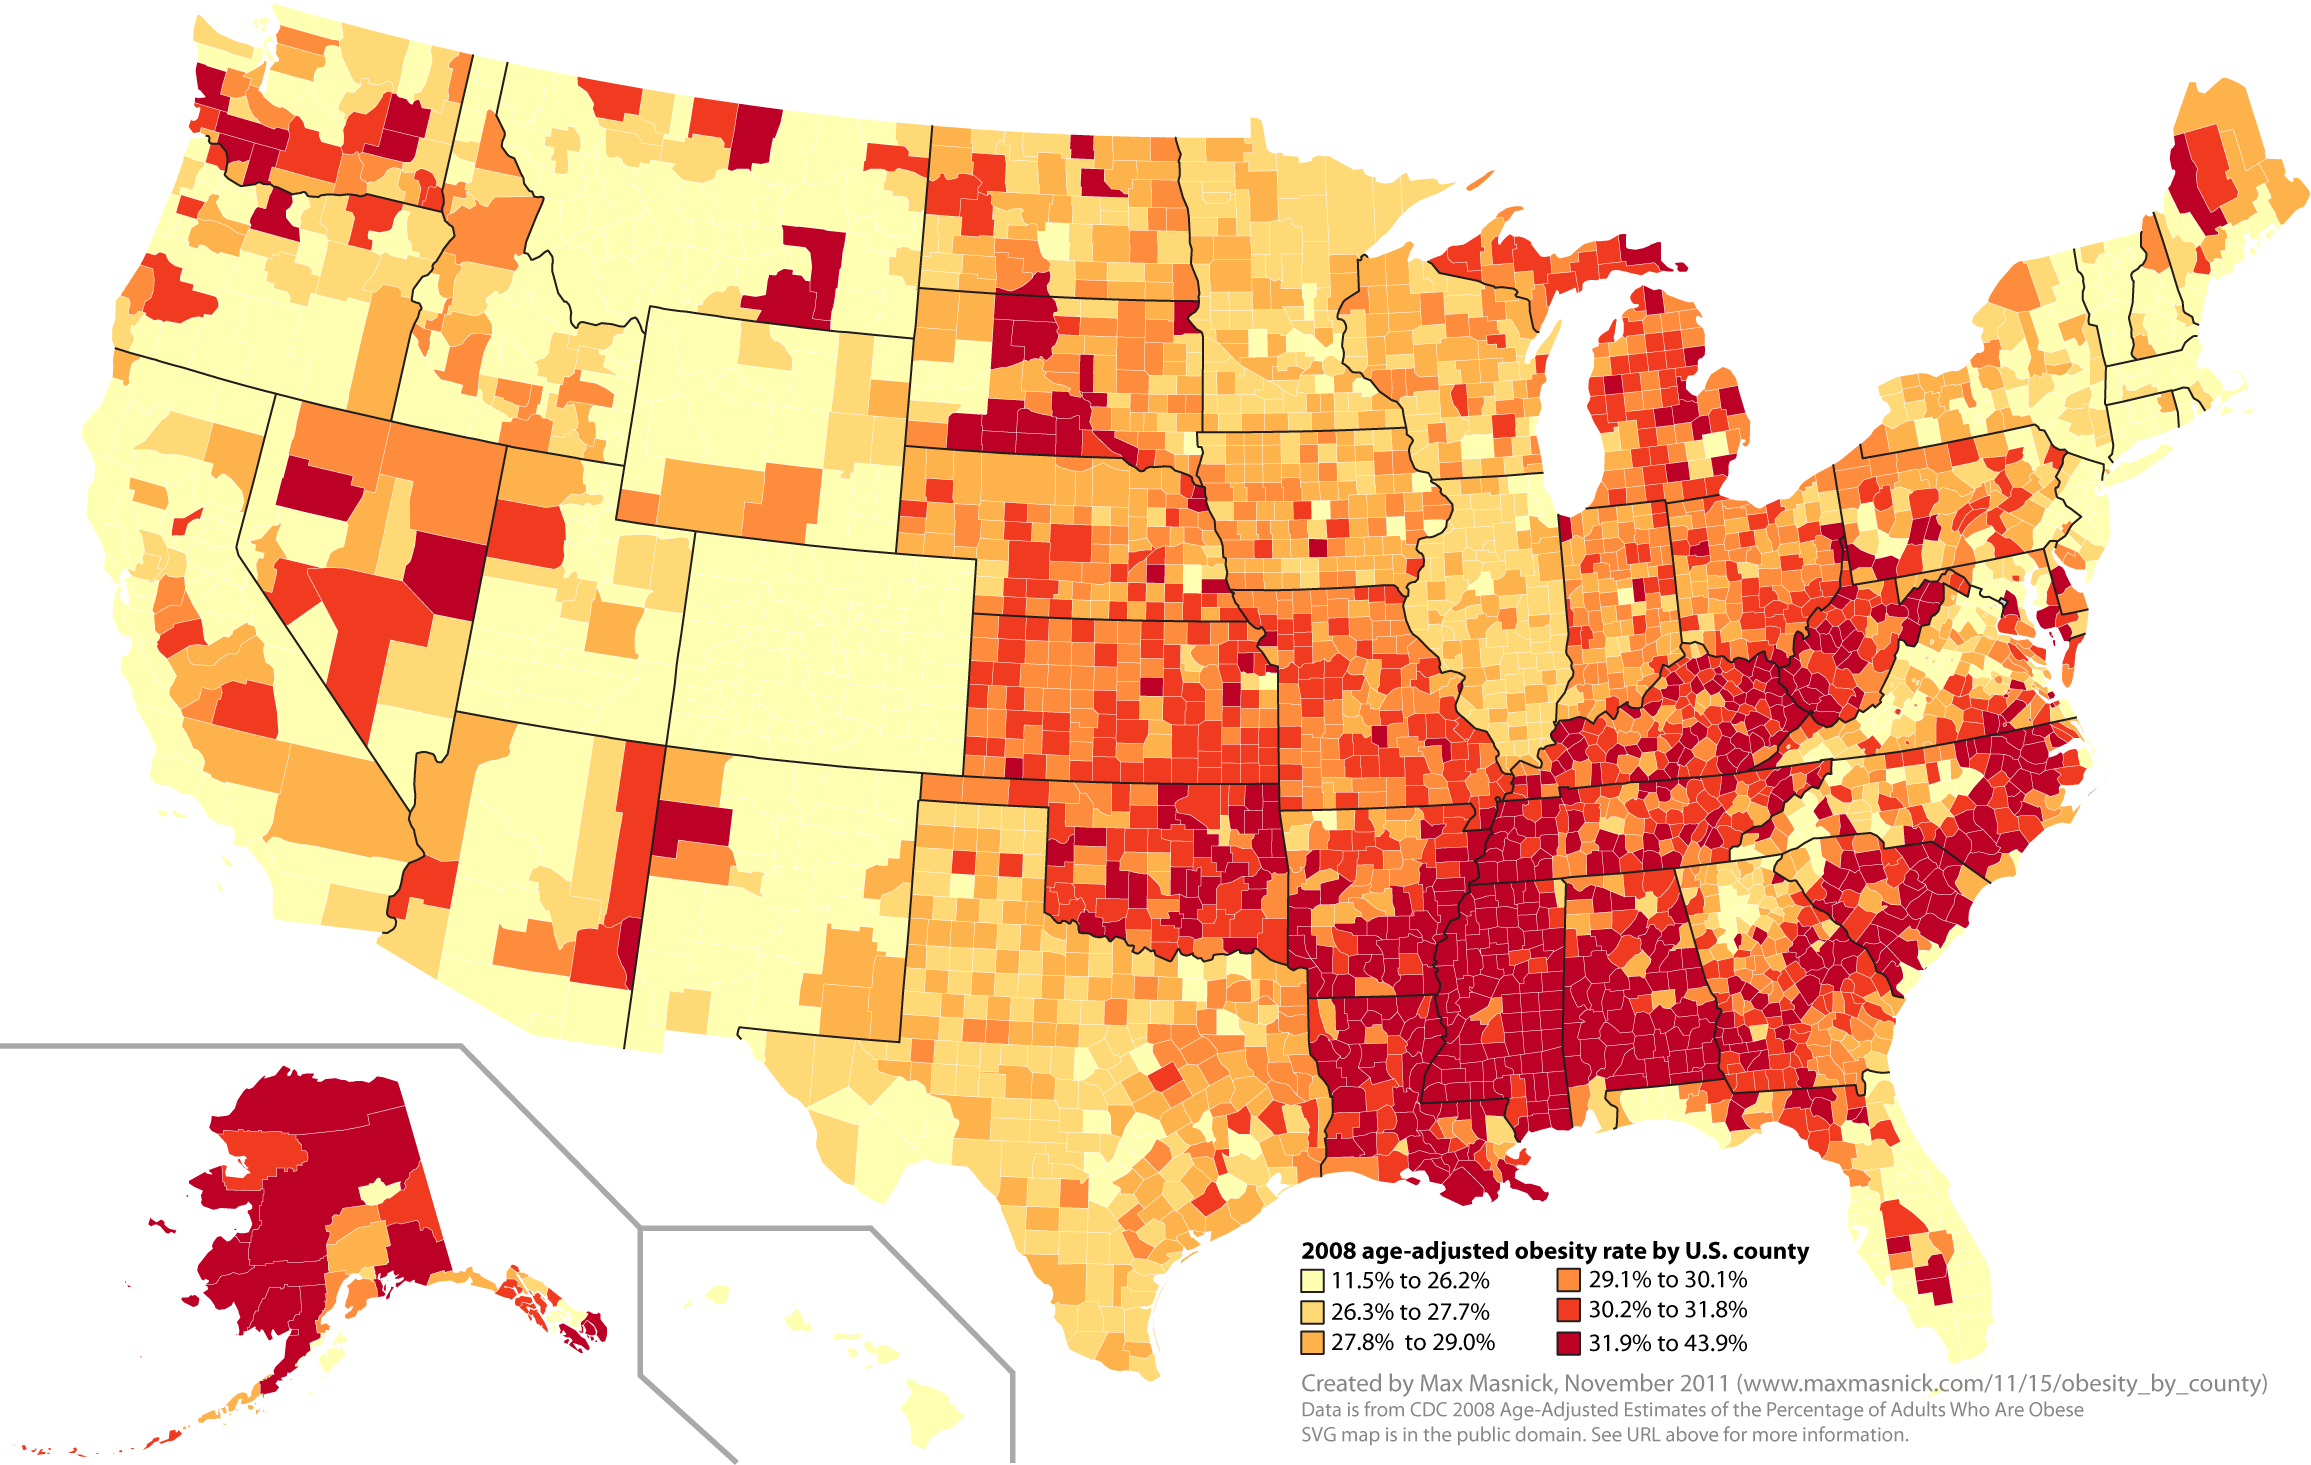
\includegraphics[width=200px]{obesity_by_county_large}
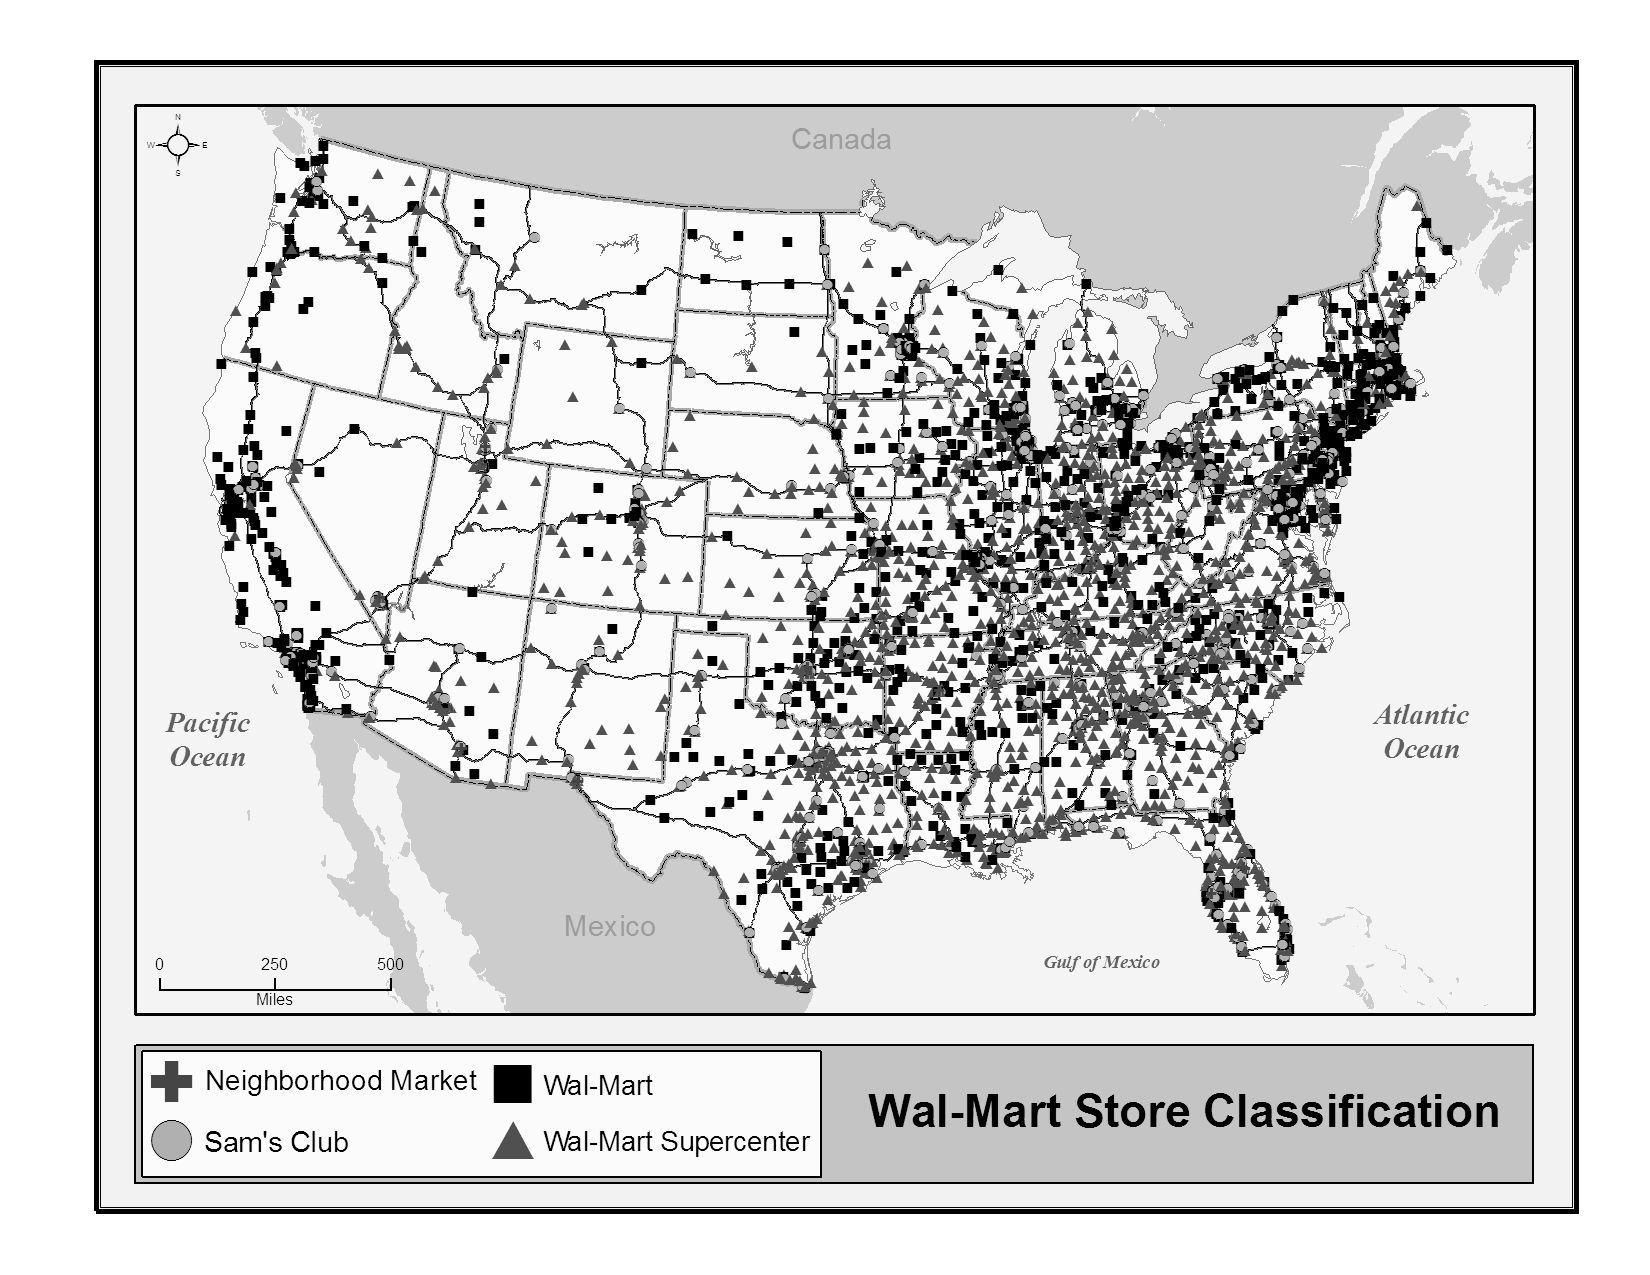
\includegraphics[width=200px]{walmartdistribution}

At first glance, there appears to be a clear correspondence between the density of Wal-Mart stores and the rate of obesity for a given area.  The match is imperfect and the actual relationship, if any, cannot be gleaned from these images alone but it does provide adequate motivation for us to explore the quality and degree of their relationship through econometric methods.  Although not shown here because of space constraints, the pattern of correspondence appears to hold over time as well.  
\subsection{Obesity}

The definition of obesity varies, but a Body-Mass-Index (BMI) of 30 kg/m is a typical value for differentiating those who are obese from those who are not.  Using this criteria, 78 million adults and 12.5 million children in the United States are obese.  A person with a BMI between 30 and 35 can expect to pay \$1850 more per year in medical expenses than a non-obese person, between 35 and 40 the cost rises to \$3086 more per year and \$5530 per year for those with a BMI above 40.  For comparison, those who smoke pay \$1274 per year more than non-smokers.\footnote{Sharon Begley. The Costs of Obesity. Huffington Post. 30 APR 2012}  Further, obesity is linked to high blood pressure, diabetes, stroke and heart disease. \footnote{Charles Courtemanche. Supersizing Supercenters? The Impact of Wal-Mart Supercenters on Body Mass Index and Obesity. Journal of Urban Economics, Elsevier, vol. 69(2), pages 165-181, March.} The Mayo clinic lists the following as risk factors for obesity:  genetics, lifestyle, diet, smoking, pregnancy, lack of sleep, medications, age, socioeconomic factors, and medical problems.\footnote{Source: http://www.mayoclinic.com/health/obesity/DS00314/DSECTION=risk-factors}  
\subsection{Wal-Mart Stores, Inc.}

The first Wal-Mart store opened in Rogers, Arkansas in 1962. By focusing on dominating the retail space in towns with less than 50 thousand people, Wal-Mart grew to become the nation's largest retailer in 1990.  Three years later, the company had its first "billion dollar week."  It topped the Fortune 500 list for the first time in 2002 and now has 2.2 million employees, 200 million customers per week and more than 10,000 stores world-wide.\footnote{Source: http://corporate.walmart.com/our-story/heritage/history-timeline} In 1988, Wal-Mart opened the first "Supercenter" which included full service groceries.

The opening of a Wal-Mart store has a number of complex, interacting economic consequences and the net effect is truly difficult to quantify.  In rural areas, Wal-Mart's deeply discounted prices and the variety of products available for sale may truly be a boon for the local economy.  In many cases, retail sales are being reallocated - as much as 25 million dollars annually - from other businesses, many of which close or downsize.  Over the course of twenty years, the local economy may produce as much as 13 million dollars less in total output.\footnote{David Mielach. What It Really Costs When Wal-Mart Comes to Town. Businessweek Daily. 23 Apr 2012.}

Certainly, the decisions Wal-Mart makes in selecting products for its shelves has an impact multiplied over its hundreds of millions of customers per week.
\endgroup
\begingroup
	\section{Literature Review}\hfill\\
		\let\clearpage\relax
			\fontsize{12bp}{14bp}\selectfont
In "Supersizing Supercenters? The Impact of Wal-Mart Supercenters on Body Mass Index", Professor Courtmanche at the University of North Carolina notes that prior research has linked technological progress and the rise of obesity.  As the overall price of food drops, the consumption of food increases.  Because Wal-Mart has invested heavily in logistics and has strong pricing power with its vendors, he reasons that we should find evidence that obesity rates rise in a location after a Wal-Mart store opens.  Indeed, he found that the average BMI rises by 0.25 units and the obesity rate rises by 2.4\% within ten years of the store opening.  Further he finds that approximately 11\% of the rise in obesity since the late 1980s can be attributed to the proliferation of Wal-Mart stores.\footnote{Charles Courtemanche. Supersizing Supercenters? The Impact of Wal-Mart Supercenters on Body Mass Index and Obesity. Journal of Urban Economics, Elsevier, vol. 69(2), pages 165-181, March.}
			
\endgroup
\begingroup
	\section{Theoretical Framework}\hfill\\
		\let\clearpage\relax
			\fontsize{12bp}{14bp}\selectfont
\subsection{Data Overview}
We used county level data for the United States, excluding counties in Virginia, Alaska, and Hawaii.  All of the variables that were percentages take on values that are between 0 and 100, not between 0 and 1. Our single dependent variable {\textit{pct\_obese}} (Percentage of adult obesity in a county) came from the University of Wisconsin�s 2013 County Health Rankings. Our primary explanatory variable was {\textit{wm_pertenthou}} (Walmart stores per 10,000 residents in a county). The location for each Walmart came from GPS Points-of-Interest data. The variable {\textit{ wm_per_sq }} is the squared term of our primary explanatory variable; it measures if there is an increasing or decreasing marginal effect. Data from the Bureau of Economic Analysis was used to control for employment factors. We used 2011 estimates from the U.S. Census Bureau to control for demographic factors such as education, age, gender, and ethnicity. See tables A.1 and A.2 in appendix for a complete list of all of our explanatory variables and their summary statistics, respectively.
			\begin{samepage}
\subsection{OLS Model}
We estimated the effect of the concentration of Wal-Mart stores on the percent of people obese in a county with the following equation:\\
\fontsize{8bp}{10bp}\selectfont
\begin{dmath}
PCT\_OBESE = \beta_{0} + \beta_{1}(WM\_PER\_TENTHOU) + \beta_{2}(WM\_PER\_SQ) + \beta_{3}(PCI)  + \beta_{4}(MEDIAN\_HOUSE\_INC) + \beta_{5}(PCT\_POVERTY) + \beta_{6}(PCT\_UNEMPLOY) + \beta_{7}(PCT\_FARM\_JOBS) + \beta_{8}(TRAVEL\_TIME\_WORK) + \beta_{9}(PCT\_UNINSURED) + \beta_{10}(PCT\_HS) + \beta_{11}(PCT\_COLLEGE) + \beta_{12}(PCT\_FASTFOOD) + \beta_{13}(PCT\_DRINKING) + \beta_{14}(PCT\_SMOKING) + \beta_{15}(PCT\_UNDER\_5) + \beta_{16}(PCT\_UNDER\_18) + \beta_{17}(PCT\_OVER\_65) + \beta_{18}(PCT\_FEMALE) + \beta_{19}(PCT\_BLACK) + \beta_{20}(PCT\_AMIND) + \beta_{21}(PCT\_ASIAN) + \beta_{22}(PCT\_PACISLAND) + \beta_{23}(PCT\_HISPANIC) + \beta_{24}(PCT\_FOREIGN\_BORN) + u
\end{dmath}
\end{samepage}
			
\endgroup
\begingroup
	\section{Results}\hfill
		\let\clearpage\relax
			\fontsize{12bp}{14bp}\selectfont

The high R-squared and adjusted R-squared (0.64 and 0.63, respectively) indicate that the
model explains a significant portion of the variation in the pct_obese variable. The Breusch-
Pagan test found some heteroskedasticity in the original model, so the regression was
executed with robust standard errors. The VIF for each variable were also analyzed to detect
multicollinearity, finding that four variables had VIF values above ten, but the average VIF was
5.90. Based on these results, we conclude that multicollinearity is not a serious problem in the
model. 
\fontsize{12bp}{14bp}\selectfont

We observe that both Wal-Mart variables are statistically significant, finding that for an
additional Wal-Mart store per 10,000 people, there is a 0.89\% increase of the percentage of
obese in the county, but a 0.45\% decreasing marginal return. We also observe that the other
significant variables in the model match our expectations regarding their relative effects on
obesity (e.g. education is negatively correlated, while poverty and access to fast good are
positively correlated).
\endgroup
\begingroup
	\section{Conclusion}\hfill\\
		\let\clearpage\relax
			\fontsize{12bp}{14bp}\selectfont
We take our results as a preliminary indicator that there exists a relationship between the presence of Wal-Mart stores and a local rise in obesity.  Our findings are supported by Courtmanche\footnote{Charles Courtemanche. Supersizing Supercenters? The Impact of Wal-Mart Supercenters on Body Mass Index and Obesity.
Journal of Urban Economics, Elsevier, vol. 69(2), pages 165-181, March.}.  We also agree with his conclusion that the main effect in play is the pricing power Wal-Mart wields over its vendors, particularly with industrial, processed foods.  As traditional grocers in a community are replaced, the aggregate diet shifts because these foods - which are linked with obesity - are more readily substituted against fresh produce.  As retail consumers, we are similar to foragers in the sense that we take from our surroundings what is most readily available.  But as Courtmanche writes, Wal-Mart is not evil.  Instead, the firm supplies what it perceives as demand by its customers.  We hope to contribute to the larger dialog a sense that we are not merely passive foragers because we have the ability to recognize hidden externalities.

The scope of our research is limited to the set of tools we acquired in the course of our first semester of econometrics and by the time allotted to explore and document our findings.  We suggest that our next steps would begin by resolving the degree to which the relationship between Wal-Mart and obesity is merely correlation.  We recognize the possibility that these two phenomenon arose independently in the southern United States: for example, they may both be products of the rapid industrialization of the South in the last half the of the 20th century.  We would also like to quantify the direct and indirect costs (i.e. increased medical costs), if any, associated with obesity that arises from the proliferation of Wal-Mart stores.  
\endgroup

\begingroup
\let\clearpage\relax
\appendix
			\section{Tables}
			\subsection{Variable List}
\includegraphics[width=0.9\textwidth]{Variables}
			\subsection{Summary Statistics}
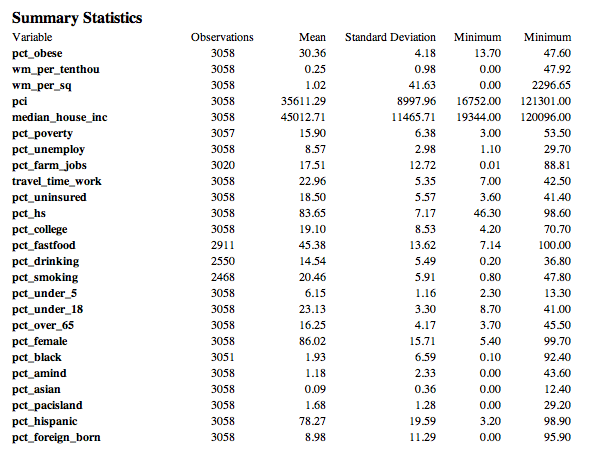
\includegraphics[width=0.9\textwidth]{sumstat}
			\subsection{Regression Results, Percent Obesity}
\fontsize{5bp}{5bp}\selectfont
\begin{tabular}{|l|l|l|}
\hline
VARIABLES & OLS & Robust Std. Errors \\      \hline 
wm\_per\_tenthou & 0.891** & 0.891** \\      \hline
 & (0.383) & (0.374) \\      \hline
wm\_per\_sq & -0.453* & -0.453** \\      \hline
 & (0.267) & (0.226) \\      \hline
pci & -1.11e-05 & -1.11e-05 \\      \hline
 & (1.19e-05) & (1.32e-05) \\      \hline
median\_house\_inc & -3.90e-05** & -3.90e-05** \\      \hline
 & (1.55e-05) & (1.61e-05) \\      \hline
pct\_poverty & 0.0691*** & 0.0691*** \\      \hline
 & (0.0238) & (0.0255) \\      \hline
pct\_unemploy & -0.194*** & -0.194*** \\      \hline
 & (0.0291) & (0.0309) \\      \hline
pct\_farm\_jobs & 0.0236*** & 0.0236*** \\      \hline
 & (0.00678) & (0.00692) \\      \hline
travel\_time\_work & 0.0134 & 0.0134 \\      \hline
 & (0.0158) & (0.0165) \\      \hline
pct\_uninsured & -0.170*** & -0.170*** \\      \hline
 & (0.0172) & (0.0187) \\      \hline
pct\_hs & -0.0630*** & -0.0630*** \\      \hline
 & (0.0186) & (0.0194) \\      \hline
pct\_college & -0.213*** & -0.213*** \\      \hline
 & (0.0150) & (0.0161) \\      \hline
pct\_fastfood & 0.0279*** & 0.0279*** \\      \hline
 & (0.00541) & (0.00562) \\      \hline
pct\_drinking & 0.00347 & 0.00347 \\      \hline
 & (0.0144) & (0.0147) \\      \hline
pct\_smoking & 0.0572*** & 0.0572*** \\      \hline
 & (0.0143) & (0.0148) \\      \hline
pct\_under\_5 & -0.0512 & -0.0512 \\      \hline
 & (0.145) & (0.156) \\      \hline
pct\_under\_18 & 0.162*** & 0.162*** \\      \hline
 & (0.0505) & (0.0544) \\      \hline
pct\_over\_65 & -0.0679*** & -0.0679** \\      \hline
 & (0.0259) & (0.0280) \\      \hline
pct\_female & -0.161*** & -0.161*** \\      \hline
 & (0.0158) & (0.0177) \\      \hline
pct\_black & -0.0630*** & -0.0630*** \\      \hline
 & (0.0132) & (0.0133) \\      \hline
pct\_amind & -0.0767* & -0.0767** \\      \hline
 & (0.0416) & (0.0356) \\      \hline
pct\_asian & -1.076*** & -1.076*** \\      \hline
 & (0.215) & (0.189) \\      \hline
pct\_pacisland & 0.0728 & 0.0728 \\      \hline
 & (0.0666) & (0.0616) \\      \hline
pct\_hispanic & 0.0647*** & 0.0647*** \\      \hline
 & (0.0152) & (0.0178) \\      \hline
pct\_foreign\_born & -0.00549 & -0.00549 \\      \hline
 & (0.0184) & (0.0196) \\      \hline
Constant & 49.02*** & 49.02*** \\      \hline
 & (2.275) & (2.397) \\      \hline
 &  &  \\      \hline
Observations & 2,245 & 2,245 \\      \hline
R-squared & 0.637 & 0.637 \\      \hline
 Adjusted R-squared & 0.633 & 0.633 \\      \hline 
%\multicolumn{3}{c}{ Standard errors in parentheses} \\      \hline
%\multicolumn{3}{c}{ *** p$<$0.01, ** p$<$0.05, * p$<$0.1} \\      \hline
\end{tabular}


			
\endgroup		

\end{doublespace}
\end{document}